\documentclass[../thesis.tex]{subfiles}
 
\begin{document}
 
\begin{figure}
    \centering
    \begin{subfigure}[b]{0.32\linewidth}
        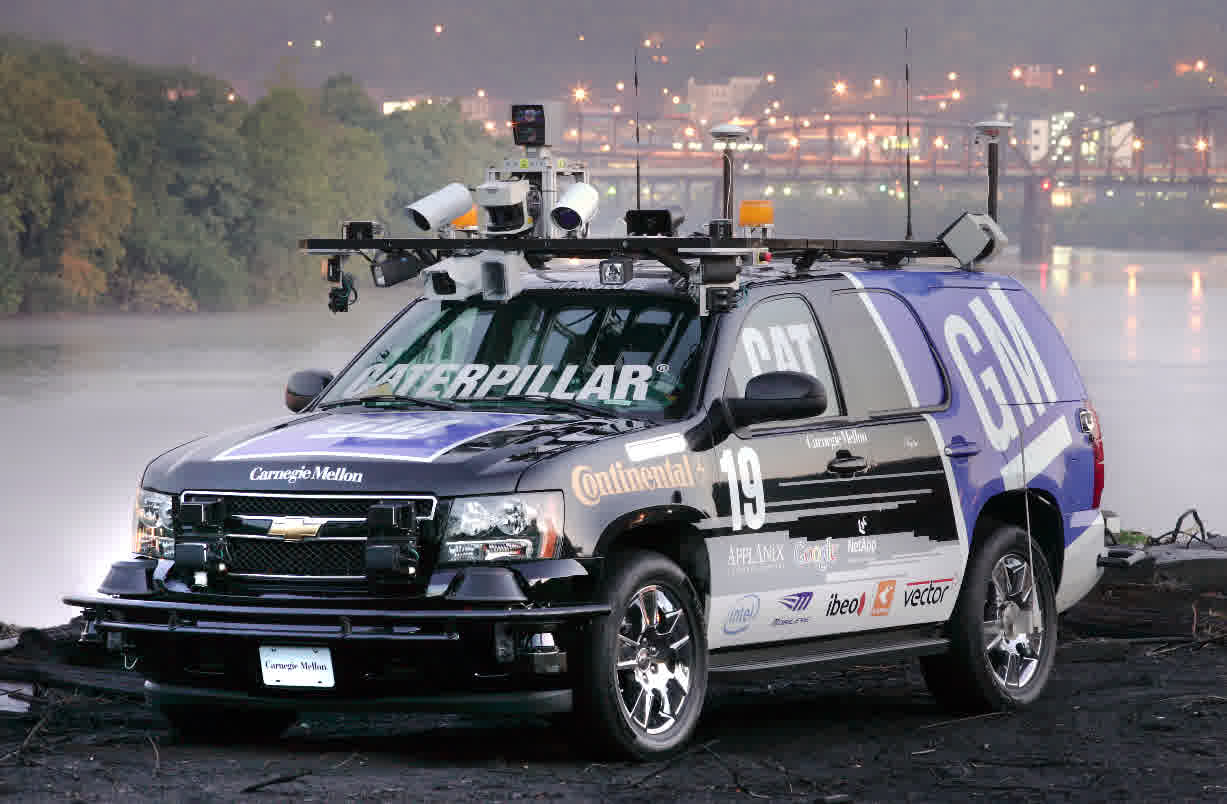
\includegraphics[height=3.5cm]{./Introduction/fig/urban_challenge.jpg}
    \end{subfigure}
    \begin{subfigure}[b]{0.32\linewidth}
        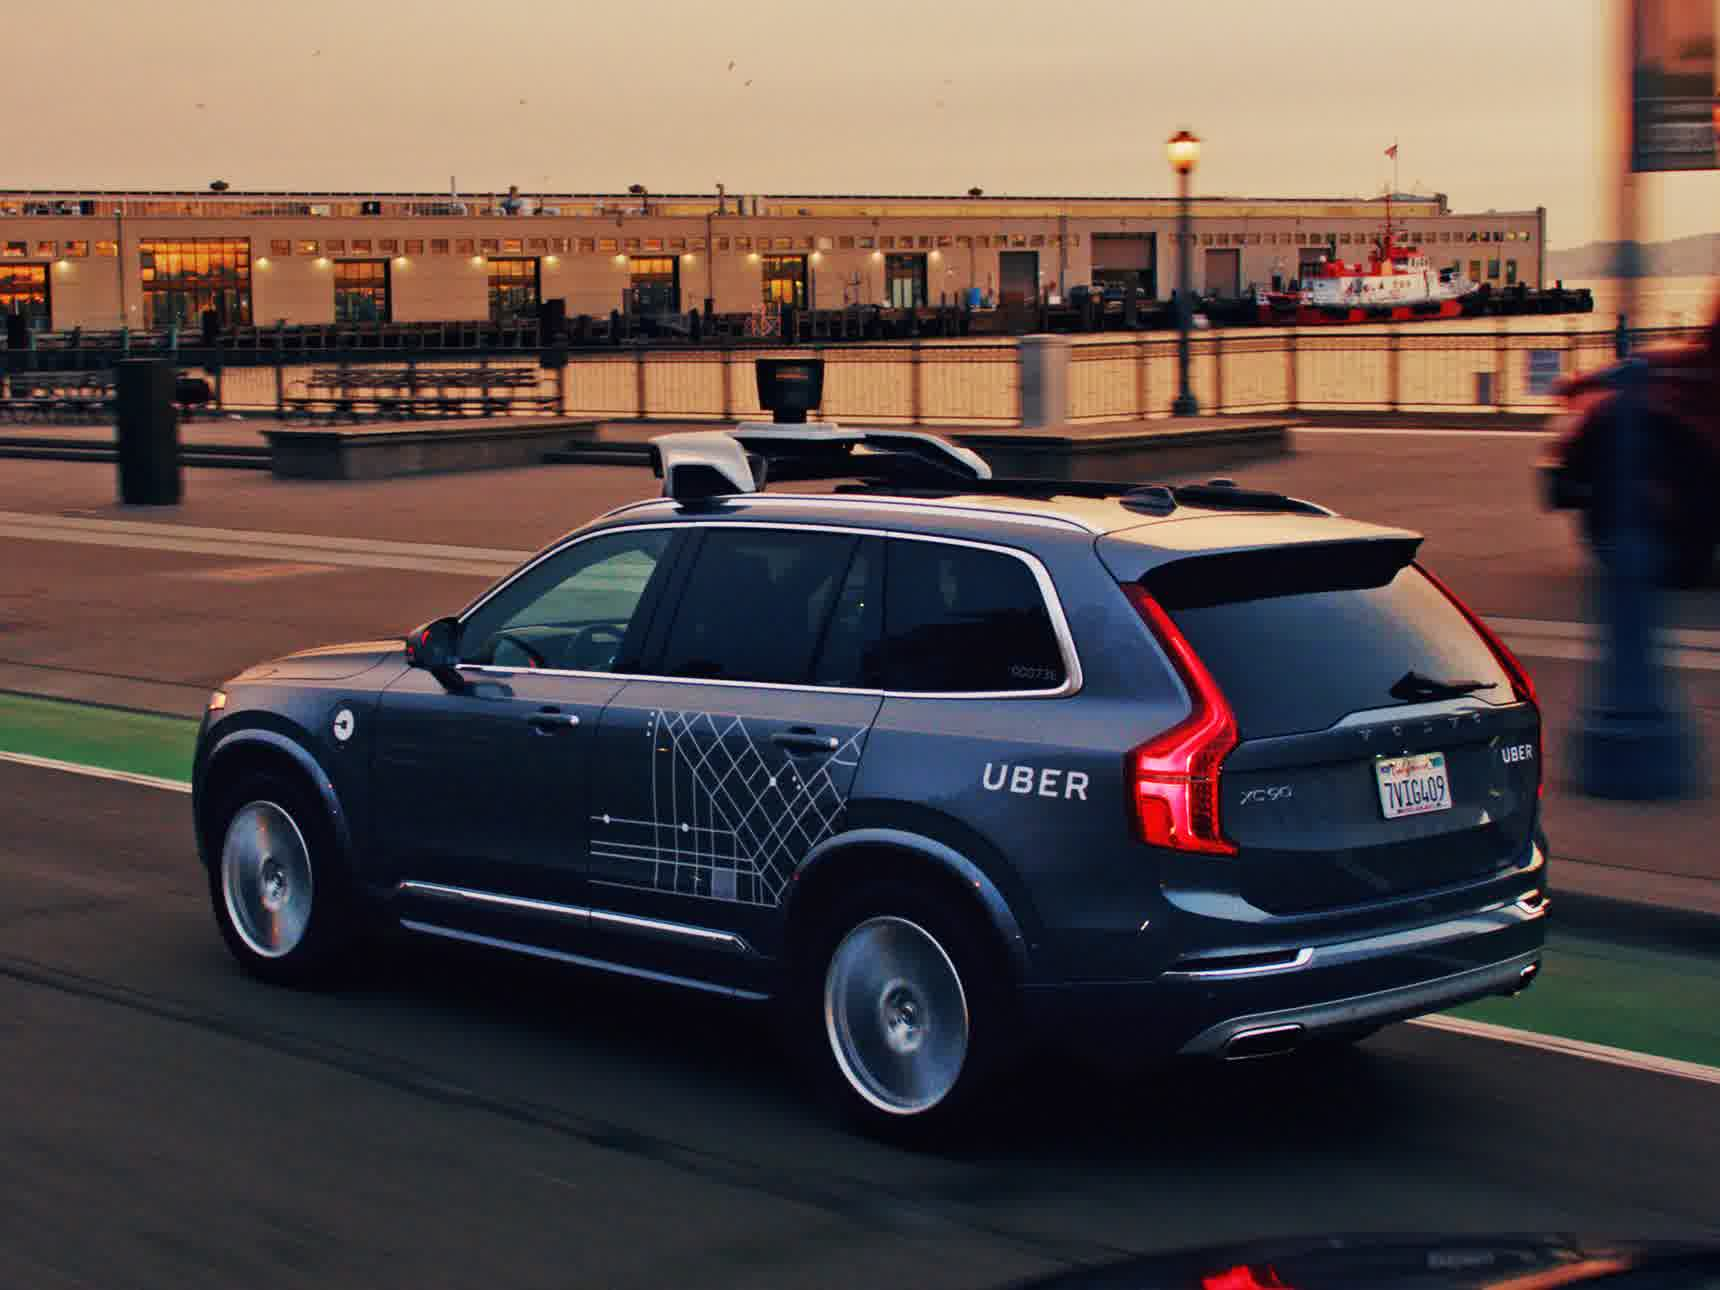
\includegraphics[height=3.5cm]{./Introduction/fig/uber.jpg}
    \end{subfigure}
    \begin{subfigure}[b]{0.32\linewidth}
        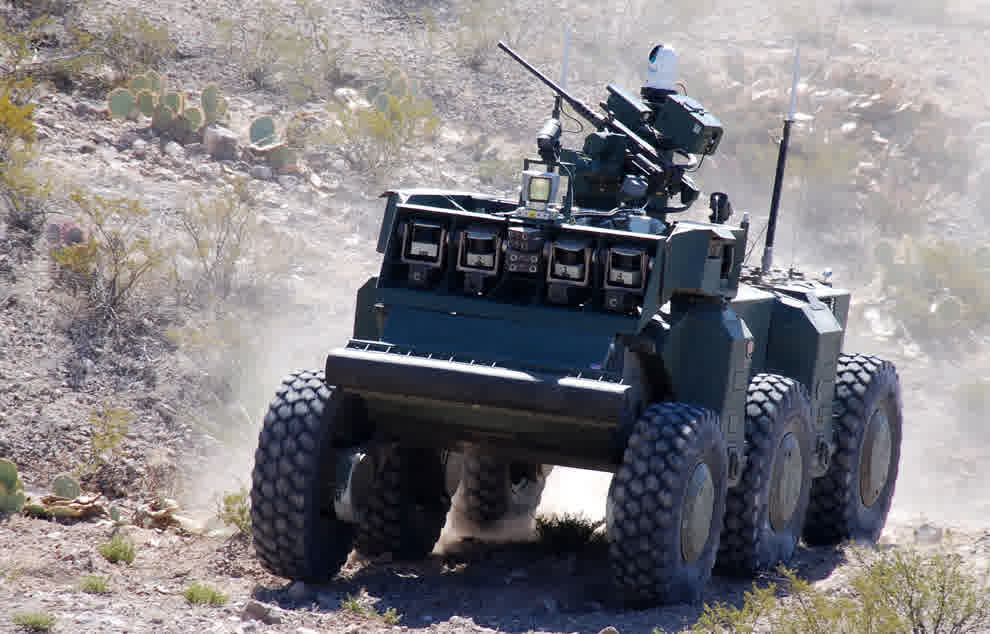
\includegraphics[height=3.5cm]{./Introduction/fig/crusher.jpg}
    \end{subfigure}
    \caption{Some well-known autonomous navigation systems: (a) The Carnegie Mellon Tartan that won the Urban Challenge in 2007 \cite{boss}. (b) Uber's self-driving vehicle. (c) Crusher. \cite{stentz2007crusher}}
    \label{fig:uber_rock}
\end{figure}
 
\section{Motivation}
 
%%%  Introduce for Motion Planning in Autonomous Navigation  %%%
 
% The rapid urbanization globally in the recent past has led to severe road congestion, a rise in pollution levels and an increase in road accidents, therefore presenting a very grim picture of the current state of urban transportation. 
% At the moment, private automobiles are widely recognized as an unsustainable solution for the future of personal urban mobility \cite{reinventing}. 
% Fortunately, however, great strides have been made in the development of autonomous driving technologies, energized by the successful demonstrations by some teams at the DARPA Urban Challenge \cite{boss, multimodaltartan}. 
% By offering an opportunity to develop sustainable and safe solutions to personal mobility \cite{usecases_of_AD}, they also hint at a complete overhaul of the urban transportation landscape by ushering in Autonomous Vehicles-on-Demand. 

In modern autonomous systems, \textit{motion planning} refers to a process where the desired movement task is broken into discrete motions that satisfy movement constraints and possibly optimize some aspect of the movement \cite{wiki:motion-planning}. 
For autonomous navigation system, the motion planning algorithm gathers information from sensors, performs optimization over the cost of the trajectory toward the desired configuration state (subjected to vehicle constraints if needed), and finally outputs the action commands for execution. 
It is worth noting that for complex decision making tasks, raw sensor information is usually processed through additional \textit{perception} module to extract informative features before entering the motion planning module.
In this viewpoint, the motion planning module stands in a crucial position throughout the decision-making pipeline in that the potential imperfect sensings, resulted from sensor noise and erroneous inferences of the perception module, are accumulated here. 
Furthermore, accurate yet efficient decisions need to be made with minimal computations.

Recently, great strides have been made in the development of autonomous driving technologies, energized by the successful demonstrations by some teams at the DARPA Urban Challenge \cite{boss, multimodaltartan}.
While there is a foreseeable trend on operating autonomous driving technologies on-road within a decade, researchers have gained interests in solving extreme/aggressive motion planning in the off-road situations or unstructured terrain \cite{kolter2010probabilistic,williams2016aggressive,gray2012predictive,cutler2016autonomous,cutler2014reinforcement}. 
This thesis investigates both traditional motion planning and alternative end-to-end learning algorithms in the off-road settings.
Specifically, we are interested in planning and learning approaches for unmanned ground vehicles in high-dimensional state space, which arise inevitably in traditional model-based planning approaches when using a more complex vehicle model, or in end-to-end learning algorithms that directly use raw sensor streams as its inputs.

\subsection{Traditional Motion Planner}
 
%%% Intro of Graph based and sample based planner %%%
 
The two most common approaches for ground vehicles motion planning are the graph-based planner and sample-based planner. 
Both approaches have shown their robustnesses in the DARPA Urban Challenge \cite{koenig2002d,kuwata2008motion} and UPI program \cite{kelly2006toward,stentz2007crusher}, where the feasible trajectories can be solved efficiently under certain reasonable assumptions. 
The output trajectories can be fine-tuned with optimization techniques to ensure criteria such as smoothness and kinematic constraints \cite{dolgov2008practical}.
 
%%% Pros and cons of two approach applied to off-road (extreme) navigation %%%
 
Though graph-based planning research has advanced significantly in recent years for the application of off-road navigation \cite{kelly2006toward,stentz2007crusher}, it is limited to the low-dimensional configuration space.
For problems that require much more complicated modeling of the dynamic systems, such as maneuvering agilely and aggressively on rough terrain, it will inevitably lead to a higher dimensional configuration space, and thus slows down the standard graph-based approaches. 
In fact, one of the main challenges for off-road motion planning comes from the fact that the vehicle dynamics are much more unpredictable in contrast to on-road conditions. 
Factors such as wheel-terrain interaction for modeling the sliding effect is still an active research area \cite{shibly2005equivalent,rubinstein2004detailed}. 
% Maneuvering agilely and aggressively on rough terrain requires a more complex vehicle model, which inevitably leads to a higher dimensional configuration space, and thus slows down the standard graph-based approaches. 
 
 
Sample-based planners, on the other hand, are more efficient in solving higher-dimensional motion planning. 
Built upon the successful application of randomized approaches to many robotics problems such as manipulation \cite{kuffner2000rrt}, researchers have tried to extend the approaches to provide aggressive motion planning for vehicles that exhibit dynamics behaviors such as drifting  \cite{hwan2011anytime}. 
However, unlike graph-based planners that guarantee a certain level of optimality, sample-based planners in general only permit asymptotic convergence to the optimal solution. 
Moreover, it is not straight-forward to implement in kinodynamic planning problems.
 
%%% Summary of the traditional motion planner (Link to end-to-end in the next section) %%%
 
Despite the pros and cons of each approach, they both share a common framework where an intelligent pipeline is built to efficiently gather incoming sensor data and take suitable control actions with good repeatability and fault-tolerance. 
The resulting autonomous navigation system is addressed in a modular fashion, where specialized algorithms are developed for each subsystem and finally integrated with some fine tunings.
 
 
\subsection{Learning End-to-end Controller}
 

%%% Intro of end-to-end learning  %%%
%%%  Our choice of using DRL instead of RL  %%%
 
More recently, however, there is an interest in applying an end-to-end approach wherein one can learn a complex mapping that goes directly from the input (e.g., camera images or laser scan measurements) to the output (e.g., steering and throttle commands) by leveraging the availability to a large volume of task-specific data. 
% This approach is purported to perform better since we are optimizing the whole system. 
The end-to-end approaches have become more appealing with the use of deep learning in robotics and have shown successes in developing visuomotor policies for autonomous driving \cite{deepdriving,nvidiacar,endtoendcars}. 
However, the traditional deep supervised learning-based driving requires a great deal of human annotation and may not be able to deal with the problem of accumulating errors \cite{ross2011reduction}. 

On the other hand, deep reinforcement learning (DRL) offers a better formulation that allows policy improvement with feedback, and has achieved human-level performance on several video games \cite{mnih2013playing, mnih2015human,2016-TOG-deepRL}.
The choice of DRL over the more tried and tested waters of supervised learning comes from the interest of better generalization and allowing for a more exploration-friendly setting. 
Recently, there have been great demands and improvements on realistic simulators \cite{deepdrive,udacity} with the hope that the acquired learning in such a simulator can be transferable to the real world with minimal tuning \cite{you2017virtual}. 
 
\begin{figure}[t]
    \centering
    \begin{subfigure}[b]{0.45\linewidth}
        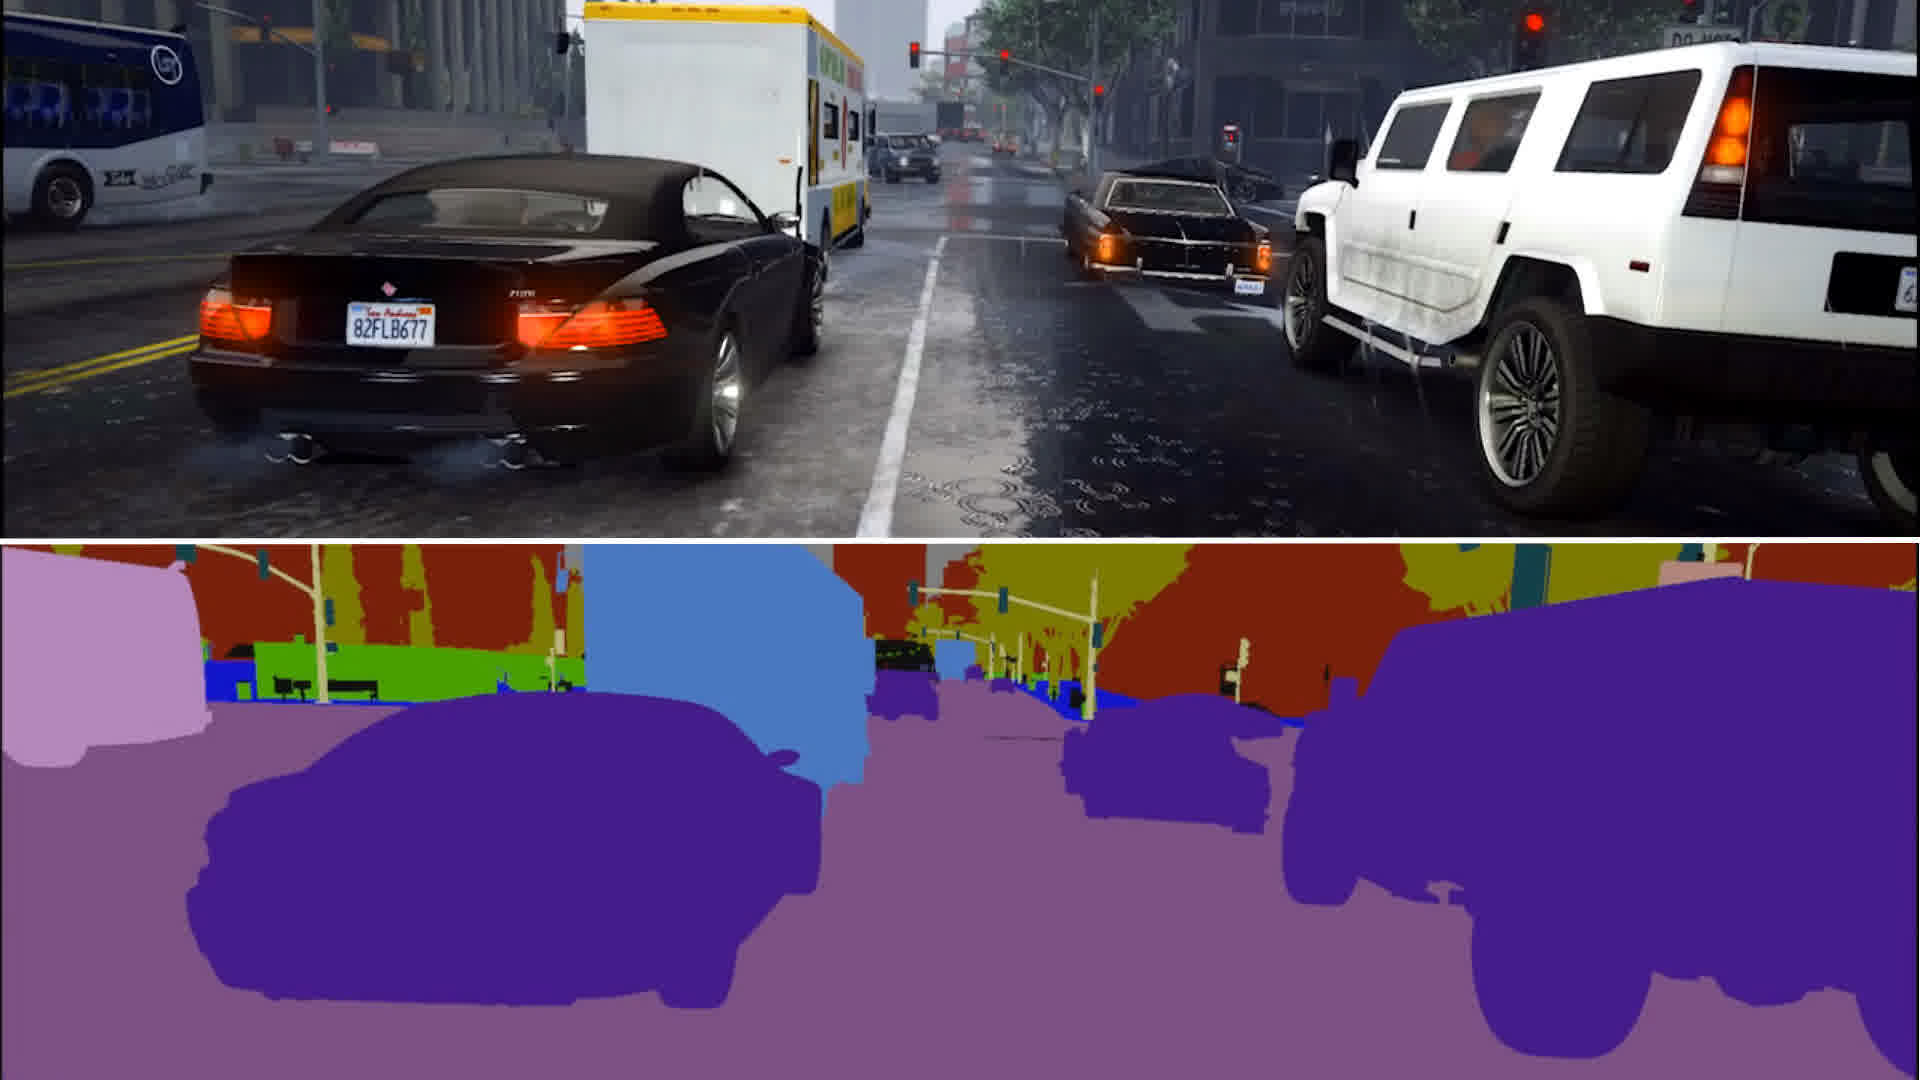
\includegraphics[height=4cm]{./Introduction/fig/gta.jpg}
    \end{subfigure}
    \begin{subfigure}[b]{0.45\linewidth}
        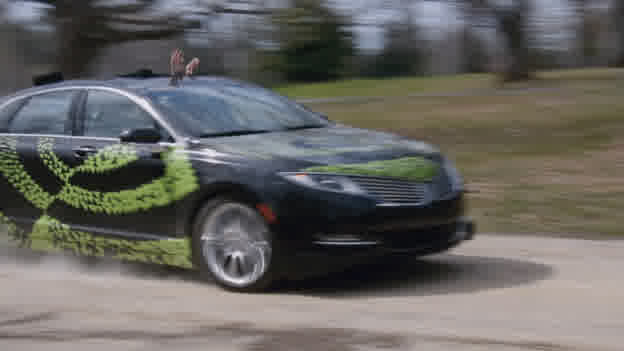
\includegraphics[height=4cm]{./Introduction/fig/nvidia.jpg}
    \end{subfigure}
    \caption{Demonstrations of the end-to-end approach on autonomous navigation applied to (a) the realistic simulator (GTA V), and (b) the full-size vehicle by NVIDIA\cite{nvidiacar}.}
    \label{fig:end-to-end}
    \vskip -0.15in
\end{figure}

\begin{figure}[b]
    \vskip -0.1in
    \centering
    \begin{subfigure}[b]{0.45\linewidth}
        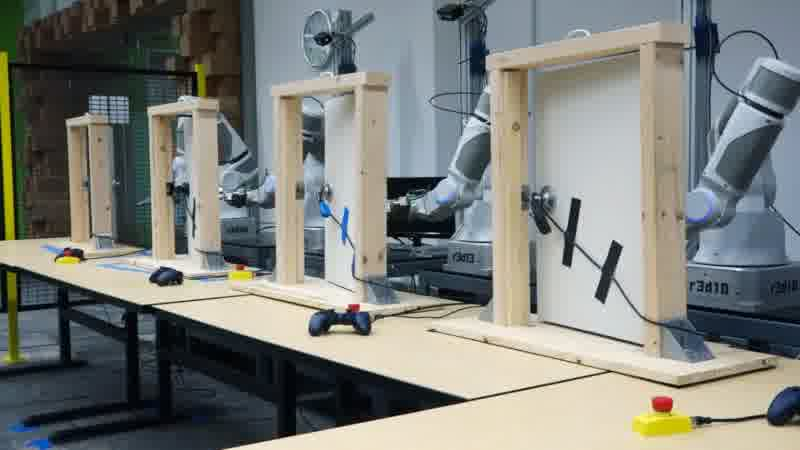
\includegraphics[height=3.5cm]{./Introduction/fig/drl_manipulation.jpg}
    \end{subfigure}
    \begin{subfigure}[b]{0.45\linewidth}
        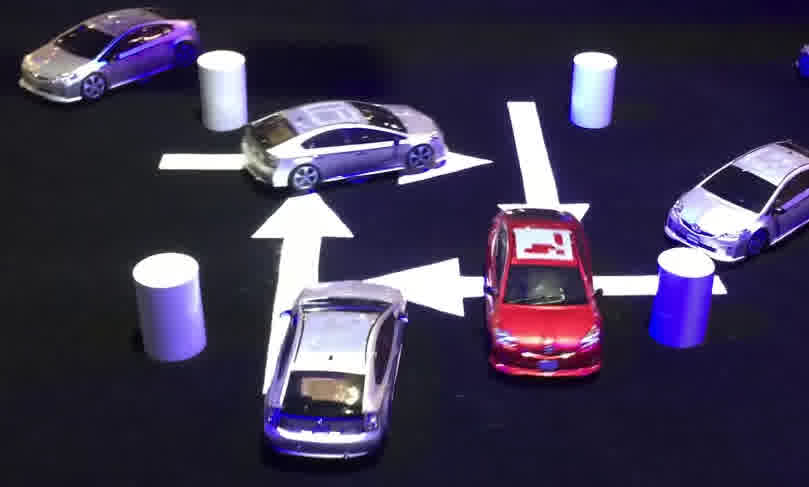
\includegraphics[height=3.5cm]{./Introduction/fig/drl_perfer_network.jpg}
    \end{subfigure}
    \caption{Recent successes on applying deep reinforcement learning (DRL) algorithms to real-world robotics problems: (a) manipulation \cite{gu2016deep}. (b) autonomous navigation. \cite{prefernetwork}}
    \label{fig:end-to-end}
\end{figure}

%%% Previous works on Multimodal DRL %%%
 
Previous work in DRL predominantly learned policies based on a single input modality, \textit{i.e.}, either low-dimensional physical states or high-dimensional pixels. 
For autonomous driving where enhancing safety and accuracy to the maximum possible extent is a top priority, developing policies that operate with multiple inputs is the need of the hour. 
In this light, several recent works in DRL have tried to solve the complex robotics tasks such as human-robot-interaction \cite{qureshi2016robot}, manipulation \cite{levine2016end}, and maze navigation \cite{mirowski2017a} with multi-sensor inputs. 
It is worth mentioning that though \citet{mirowski2017a} uses multi-sensor inputs to navigate through a maze, information such as depth is only used as an auxiliary loss, \textit{i.e.} it is not an input to the trained policy but is only used to improve the learning outcomes. 
In fact, \citet{mirowski2017a} points out that the naive RGBD policy performs worse than predicting depth as a regression task.

%%% Sensor Fusion on Multimodal DRL %%%
Our observation is that though these end-to-end learning approaches have a great potential to handle high-dimensional state space, in the multi-sensor setting the learned policy may either become over-dependent on partial sensor subset or rely heavily on all the inputs to the extent that it fails completely if a single sensor becomes unreliable.
To be clear, in the space of end-to-end sensorimotor control, the \textit{sensor fusion} outlook, as an indispensable technique to improve accuracy and robustness in a modern autonomous navigation system, has received limited attention. 
In fact, multimodal perception is an integral part of autonomous navigation solutions and even played a critical role in their success \cite{multimodaltartan} before the advent of end-to-end deep learning based approaches. 
It offers several advantages, namely robustness to individual sensor noise/failure, improved object classification and tracking \cite{elfring2016multisensor, cho2014multi, darms2008classification}, robustness to varying weather and environmental conditions, etc. 
This problem is critical as a further step toward the real-world robotics application given the current state-of-the-art DRL agents on many realistic simulators.

 

 
 
\section{Approaches}
 
In this thesis, we first propose a model-based local planner that solve the optimal kinodynamic motion planning problem. 
The local planner is built upon a vehicle model that captures important state for off-road navigation such as lateral velocity. 
Practical problems such as re-planning and optimization are addressed under the standard sample-based approach but modified appropriately to encourage a more aggressive maneuvering. 
The resulting model-predictive planner is tested on the full-size All-Terrain Vehicle (ATV) in the off-road conditions.
 
We also present an alternative end-to-end controller that uses multi-sensor input to learn an autonomous navigation policy in a physics-based gaming environment called TORCS \cite{wymann2000torcs}. 
To show the effectiveness of multimodal perception, we pick two popular continuous action DRL algorithms, namely Normalized Advantage Function (NAF) \cite{CDQN} and Deep Deterministic Policy Gradient (DDPG) \cite{DBLP:journals/corr/LillicrapHPHETS15}, and augment them to accept multimodal inputs. 
Though a multimodal sensor policy may improve the reward of the agent, it provides no guarantees on the sensitivity of the trained policy to each sensor module.
% rely heavily on all the inputs to the extent that it may fail completely even if a single sensor broke down fully or partially. 
This undesirable consequence renders sensor redundancy useless. 
To ensure that the learned policy does not succumb to such over-fitting, we apply a novel stochastic regularization method called \emph{Sensor Dropout} during training. 
Our approach reduces the policy sensitivity to a particular sensor subset and makes it capable of functioning even in the face of partial sensor failure. 
Based on the Sensor Dropout, we further embedded the standard DRL loss with an auxiliary loss that helps reduce the action variations of the multimodal policy. 
% As far as we know, we are the first to address the multimodal policy learning regarding sensor fusion.
 
Note that both the traditional and the end-to-end planner require the cost/reward heuristic function to guide the policy and formally define the optimization problem. 
However, unlike in the urban environment where cost function can be well defined in a rule-based structure, finding a cost function for off-road navigation can be non-trivial and often requires lots of handy tunings. \cite{silver2010learning}
Here, motivated by the recent successes \cite{wulfmeier2015maximum,wulfmeier2016watch}, we also investigate into the using deep neural network as a function approximator to construct the cost/reward function under deep inverse reinforcement learning (DIRL) platform. 
Again, we can leverage the availability to a large volume of task-specific data and solve the problem with minimal engineering hand-tunings.
 
To summarize, the primary contributions of this thesis are:
\begin{enumerate}
 
    \item %RRT
    Propose a model-based local planner for high-speed maneuvering in the off-road navigation application. 
    The planner uses Rapidly-exploring Random Tree (RRT) \cite{kuffner2000rrt} as its template, and is tested on a full-size all-terrain vehicle (ATV) in the off-road environment. 
    We show that the planner can perform smooth yet aggressive avoid static obstacles with high speed up to $30 kph$.
 
    \item % M-DRL
    Propose a new stochastic regularization, namely \emph{Sensor Dropout}, for training an end-to-end multi-sensor policy under deep reinforcement learning (DRL) framework. 
    The proposed method is integrated with two continuous action algorithms and heavily tested on a physics-based gaming environment called TORCS \cite{wymann2000torcs}. 
    We show that policies trained with Sensor Dropout not only perform minimal performance drop when measurements become noisy/imperfect, but are also less sensitive to any single sensing modality; therefore, makes it able to function even in the face of partial sensor failure.
 
    \item % DIRL
    Investigate into the deep inverse reinforcement learning (DIRL) algorithms that infer the cost, or traversability, of the unstructured terrain by leveraging large volume of human demonstration data collected on the field. 
    We propose two slight modifications over the current approach \cite{wulfmeier2015maximum}, including explicitly modeling the ambiguity of optimality, and integrating with failure demonstrations to overcome the spatially sparse gradient in DIRL training.
    The framework is tested on a full-size ATV in the off-road environment.
 
\end{enumerate}
 
The thesis is organized as follows:
In Chapter \ref{chap:related_work} we briefly go through the preliminary background, including the basic sample-based planner, the formal definition of deep (inverse) reinforcement learning, related stochastic regularization in the multimodal learning literature, and the two continuous action agents used in this work.
In Chapter \ref{chap:rrtplanner} we formulate our model predictive planner, followed with the derivation of the vehicle model, detailed planner design for optimal planning, and finally the experimental results on the field.
In Chapter \ref{chap:multimodalDRL} we propose a new technique at the aspect of sensor fusion to improve the performance of the end-to-end controller with multi-sensor inputs. 
In Chapter \ref{chap:dirl} we investigate the traversability analysis with the recently popular studies on deep inverse reinforcement learning.
Finally, we conclude the work in Chapter \ref{chap:conclusion} and address some of the interesting directions for future works.
 
\end{document}
